% 第6章第7节：谱划分（图划分问题与割的表示、RatioCut谱方法、NCut谱方法）。

\section{谱划分}
\label{sec:graph-spectral-partition}

最后回到章首的第三个问题：按连接强弱把顶点分成两组。本节固定$n\geq2$，要求两组都非空。先用指示向量把跨组边权写成拉普拉斯的二次型，说明只最小化跨组边权为什么会得到失衡的划分；再分别按顶点数和连接体积引入平衡，把离散问题写成Rayleigh商，放宽取值限制后用谱展开求解。连续解给出下界和候选分组，但它本身不是分组，二者要始终分开。

\subsection{图划分问题与割的表示}
\label{sec:graph-spec-partition-problem}

把顶点集分成$S$与$\bar S=V\setminus S$两组，跨组的连接强度用
\[
 \operatorname{cut}(S,\bar S)=\sum_{i\in S}\sum_{j\in\bar S}w_{i,j}
\]
衡量。这沿用了第~\ref{sec:graph-max-flow}节割的想法：把顶点分到两侧，累计跨过两侧的边上的数值。区别在于这里的图是无向的，没有源和汇，两个方向不加区分。

割权可以写成二次型。令$\bm s$为$S$的指示向量，$s_i=1$（$i\in S$）或$0$（$i\in\bar S$）。代入能量式~\eqref{eq:graph-spec-dirichlet-energy}，两端在同一组的边$(s_i-s_j)^2=0$，跨组的边$(s_i-s_j)^2=1$，所以
\begin{equation}
 \bm s^{\top}\bm L\bm s=\sum_{\{i,j\}\in E}w_{i,j}(s_i-s_j)^2=\operatorname{cut}(S,\bar S).
 \label{eq:graph-spec-cut-quadratic}
\end{equation}
于是划分问题变成在取值为$0$或$1$的向量上最小化$\bm L$的二次型。

只最小化割权并不够。若允许空组，$S=\varnothing$的割权为零，问题平凡；这正是要求两组非空的原因。即使要求非空，最小割也常常只切下一个连接很弱的顶点。图~\ref{fig:graph-spec-cut-indicator}中两个单位权三角形由一条单位权边相连，顶点$7$以权$0.6$挂在顶点$2$上。直观的分法是沿中间的桥切开，割权为$1$；但只切下顶点$7$的割权是$0.6$，枚举全部$63$种非空二分可知它就是最小割。单纯的割权不关心两组各有多大。

\begin{figure}[!htb]
  \centering
  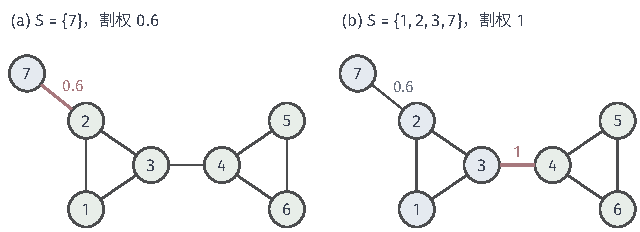
\includegraphics[width=108mm]{figures/01-basic-mathematics/04-graphs/tikz/c6-cut-indicator/figure.pdf}
  \caption{割与指示向量。两个单位权三角形由桥$\{3,4\}$相连，顶点$7$以权$0.6$连到顶点$2$。蓝色顶点属于$S$（指示向量取$1$），绿色顶点属于$\bar S$（取$0$），红色边跨组，$\bm s^{\top}\bm L\bm s$等于红色边权之和。(a)~$S=\{7\}$，割权$0.6$，是全部非空二分中的最小割；(b)~$S=\{1,2,3,7\}$，割权$1$，两组大小相近。}
  \label{fig:graph-spec-cut-indicator}
\end{figure}

\paragraph{松弛给出的上下界}
下面两小节都采用同一种论证，这里先把逻辑说清。设离散问题在有限可行集$\mathcal F$上最小化目标$J$，最优值为$J^\star$。若把可行集扩大为$\mathcal C\supseteq\mathcal F$，并把$J$延拓到$\mathcal C$上，可选的对象只多不少，最小值只能下降：$L=\min_{\mathcal C}J\leq J^\star$。这种做法称为\term{连续松弛}（continuous relaxation），它给出下界。另一方面，从连续解出发构造任意一个合法分组并计算原目标值$U$，则$U\geq J^\star$，它给出上界。于是
\[
 0\leq U-J^\star\leq U-L ,
\]
差$U-L$限制了所得分组可能的次优程度。它只是次优程度的上界，只有下界恰好取到$J^\star$时才等于真实的差距。

\subsection{RatioCut谱方法}
\label{sec:graph-spec-ratio-cut}

为了不让一组过小，把割权按两组的顶点数放大。设$a=|S|>0$，$b=|\bar S|>0$，定义\term{比率割}（RatioCut）
\begin{equation}
 \operatorname{RatioCut}(S,\bar S)=\operatorname{cut}(S,\bar S)\Bigl(\frac1a+\frac1b\Bigr).
 \label{eq:graph-spec-ratio-cut}
\end{equation}
一组越小，$\frac1a$越大，切下它的代价就越高。在图~\ref{fig:graph-spec-cut-indicator}中，只切下顶点$7$的RatioCut为$0.6\cdot(1+\tfrac16)=0.7$，沿桥切开的RatioCut为$1\cdot(\tfrac14+\tfrac13)=\tfrac7{12}\approx0.58$；枚举可知后者是全部非空二分中的最小值。

\paragraph{两水平向量}
接下来把RatioCut写成Rayleigh商。对给定分组构造在两组上分别取常数的向量
\begin{equation}
 f_i=\sqrt{b/a}\quad(i\in S),\qquad f_i=-\sqrt{a/b}\quad(i\in\bar S).
 \label{eq:graph-spec-ratio-cut-vector}
\end{equation}
逐项计算：$\bm1^{\top}\bm f=a\sqrt{b/a}-b\sqrt{a/b}=\sqrt{ab}-\sqrt{ab}=0$；$\bm f^{\top}\bm f=a\cdot\tfrac ba+b\cdot\tfrac ab=n$；跨组边上的差都是$\sqrt{b/a}+\sqrt{a/b}=n/\sqrt{ab}$，同组边上的差为零，所以
\[
 \bm f^{\top}\bm L\bm f=\operatorname{cut}(S,\bar S)\frac{n^2}{ab}=n\operatorname{cut}(S,\bar S)\Bigl(\frac1a+\frac1b\Bigr)=n\operatorname{RatioCut}(S,\bar S).
\]
因此$\operatorname{RatioCut}(S,\bar S)=\bm f^{\top}\bm L\bm f/\bm f^{\top}\bm f$。最小化RatioCut，等价于在“与$\bm1$正交、只取两个由分组决定的值”的向量中最小化$\bm L$的Rayleigh商。去掉“只取两个值”的限制，只保留$\bm f\neq\bm0$与$\bm f\perp\bm1$，可行集从有限个向量扩大为一个$n-1$维子空间去掉原点，这就是连续松弛。

\begin{theorem}[RatioCut的谱下界]
\label{thm:graph-spec-ratio-cut-bound}
设$\bm L$的特征值为$0=\lambda_1\leq\lambda_2\leq\cdots\leq\lambda_n$，则
\[
 \min_{\bm f\neq\bm0,\ \bm f\perp\bm1}\frac{\bm f^{\top}\bm L\bm f}{\bm f^{\top}\bm f}=\lambda_2 ,
\]
最小值在第二特征向量$\bm u_2$处取到。因此对每个非空二分都有$\operatorname{RatioCut}(S,\bar S)\geq\lambda_2$。
\end{theorem}

\begin{proof}
$\bm1$在$\bm L$的零空间中，所以可以取标准正交特征基使$\bm u_1=\bm1/\sqrt n$。$\bm f\perp\bm1$意味着$\bm f$在$\bm u_1$上的坐标为零，$\bm f=\sum_{k\geq2}c_k\bm u_k$。由式~\eqref{eq:graph-spec-parseval}，
\[
 \frac{\bm f^{\top}\bm L\bm f}{\bm f^{\top}\bm f}=\frac{\sum_{k\geq2}\lambda_kc_k^2}{\sum_{k\geq2}c_k^2},
\]
它是$\lambda_2,\ldots,\lambda_n$以$c_k^2$为权的加权平均，不小于$\lambda_2$；取$\bm f=\bm u_2$时等于$\lambda_2$。每个两水平向量~\eqref{eq:graph-spec-ratio-cut-vector}都在可行集中，所以RatioCut不小于这个最小值。
\end{proof}

证明只用到已有的谱分解，不需要拉格朗日乘子或一般的约束优化理论。第二特征向量常称为Fiedler向量；正权支撑图连通时，由定理~\ref{thm:graph-spec-null-space}知$\lambda_2>0$。

\paragraph{从谱方向恢复分组}
连续最优解$\bm u_2$一般不是两水平向量，需要把它变回分组。既然两水平向量在$S$上取正值、在$\bar S$上取负值，自然的做法是按$\bm u_2$的坐标排序，在某个位置切开。

\begin{algorithm}[谱划分的阈值扫描]
\label{alg:graph-spec-sweep}
输入：图与谱方向$\bm v$（RatioCut用$\bm u_2$）。输出：一个非空二分及其原目标值$U$。
\begin{enumerate}
 \item 按$\bm v$的坐标从大到小排列顶点；坐标相同的顶点视为一个整体。
 \item 在相邻两个不同坐标值之间依次设阈值，坐标大于阈值的顶点组成$S$，其余组成$\bar S$，两组都非空。
 \item 对每个候选分组，用原目标（RatioCut或NCut）计算其值，保留最小者作为$U$。
\end{enumerate}
\end{algorithm}

这种逐个阈值试探的做法称为\term{阈值扫描}（threshold sweep）。扫描时不必每次重算割权：把顶点$i$从$\bar S$移入$S$时，它连向$S$的边不再跨组，连向$\bar S$的边开始跨组，所以割权增加$\sum_{j\in\bar S}w_{i,j}-\sum_{j\in S}w_{i,j}$，只需访问$i$的邻边。组大小或体积同样可以逐步更新。

\begin{figure}[!htb]
  \centering
  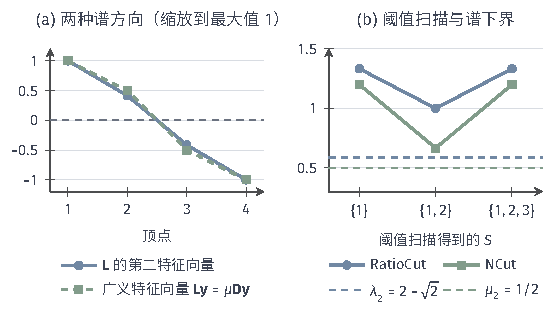
\includegraphics[width=94mm]{figures/01-basic-mathematics/04-graphs/tikz/c6-four-path-sweep/figure.pdf}
  \caption{单位权四点路径$1-2-3-4$上的两种谱划分。(a)~$\bm L$的第二特征向量（蓝）与广义特征问题$\bm L\bm y=\mu\bm D\bm y$的第二特征向量（绿），均按最大绝对值缩放到$1$；二者在零点两侧给出同样的分组，但中间两点的相对幅度不同。(b)~按坐标排序扫描三个阈值得到的原目标值，实线为RatioCut与NCut，虚线为相应谱下界$\lambda_2=2-\sqrt2$与$\mu_2=\tfrac12$；两种目标都在$S=\{1,2\}$处最小，且严格高于下界。}
  \label{fig:graph-spec-four-path-sweep}
\end{figure}

\paragraph{四点路径算例}
取单位权四点路径$1-2-3-4$。它的拉普拉斯的特征值为$0$、$2-\sqrt2$、$2$、$2+\sqrt2$，第二特征向量正比于$(1+\sqrt2,1,-1,-1-\sqrt2)^{\top}$；可以直接核对$\bm L\bm v=(2-\sqrt2)\bm v$。按坐标扫描得到三个候选分组，RatioCut依次为
\[
 S=\{1\}:\ 1\cdot\bigl(1+\tfrac13\bigr)=\tfrac43,\qquad
 S=\{1,2\}:\ 1\cdot\bigl(\tfrac12+\tfrac12\bigr)=1,\qquad
 S=\{1,2,3\}:\ \tfrac43 ,
\]
所以$U=1$。枚举全部七种非空二分，离散最优值也是$1$，在$\{1,2\}|\{3,4\}$处取到。谱下界为$\lambda_2=2-\sqrt2\approx0.586$，严格小于$1$，见图~\ref{fig:graph-spec-four-path-sweep}。这说明松弛通常不紧：这里恢复的分组恰好最优，但只凭$U-L\approx0.414$并不能确认这一点。

\paragraph{开销}
整个方法的开销分三部分。求$\bm u_2$：稠密完整特征分解需要$O(n^3)$时间、$O(n^2)$空间；大型稀疏图常用只求少数特征向量的迭代方法，其代价取决于求解器、所需精度和$\lambda_2$与$\lambda_3$的间隔，不能只因为$\bm L$稀疏就断言是线性时间。排序需要$O(n\log n)$。扫描时每个顶点移动一次，每条正权边被访问常数次，需要$O(n+m_+)$。

\subsection{NCut谱方法}
\label{sec:graph-spec-normalized-cut}

RatioCut用顶点个数衡量组的大小。另一种选择是用组内的连接总量：一组顶点的加权度之和
\[
 \operatorname{vol}(S)=\sum_{i\in S}d_i
\]
称为它的\term{体积}（volume）。设$p=\operatorname{vol}(S)>0$，$q=\operatorname{vol}(\bar S)>0$，定义\term{归一化割}（normalized cut，NCut）
\begin{equation}
 \operatorname{NCut}(S,\bar S)=\operatorname{cut}(S,\bar S)\Bigl(\frac1p+\frac1q\Bigr).
 \label{eq:graph-spec-normalized-cut}
\end{equation}
它要求两组的体积都为正。在图~\ref{fig:graph-spec-cut-indicator}中，顶点$7$的体积只有$0.6$，只切下它的NCut约为$1.04$；沿桥切开时两侧体积为$8.2$与$7$，NCut为$\tfrac1{8.2}+\tfrac17\approx0.26$，是全部非空二分中的最小值。

\paragraph{度加权的两水平向量}
与RatioCut平行，构造$y_i=\sqrt{q/p}$（$i\in S$）、$y_i=-\sqrt{p/q}$（$i\in\bar S$）。这次用度加权核对：
\[
 \bm y^{\top}\bm D\bm1=p\sqrt{q/p}-q\sqrt{p/q}=0,\qquad
 \bm y^{\top}\bm D\bm y=p\cdot\tfrac qp+q\cdot\tfrac pq=\operatorname{vol}(V),
\]
跨组边上的差为$\sqrt{q/p}+\sqrt{p/q}=(p+q)/\sqrt{pq}$，所以$\bm y^{\top}\bm L\bm y=\operatorname{cut}(S,\bar S)(p+q)^2/(pq)=\operatorname{vol}(V)\operatorname{NCut}(S,\bar S)$。于是
\[
 \operatorname{NCut}(S,\bar S)=\frac{\bm y^{\top}\bm L\bm y}{\bm y^{\top}\bm D\bm y},\qquad \bm y^{\top}\bm D\bm1=0 .
\]
与RatioCut相比，正交条件和长度都换成了度加权的版本，这正是第~\ref{sec:graph-spec-degree-inner-product}小节的度加权内积。两种方法采用了不同的平衡尺度。

\paragraph{化为对称归一化拉普拉斯}
先把谱计算限制在正度顶点$V_+$上。支撑孤点的体积为零，会让$\bm D$奇异，还会给$\bm L_{\mathrm{sym}}$带来额外的零特征向量$\bm e_v$，它们对应的并不是合法的正体积分组；孤点的处理放在下面单独说明。在$V_+$上$\bm D$正定，作坐标代换$\bm x=\bm D^{1/2}\bm y$，则
\[
 \frac{\bm y^{\top}\bm L\bm y}{\bm y^{\top}\bm D\bm y}=\frac{\bm x^{\top}\bm L_{\mathrm{sym}}\bm x}{\bm x^{\top}\bm x},\qquad
 \bm y^{\top}\bm D\bm1=\bm x^{\top}\bm D^{1/2}\bm1=0 .
\]
约束变成$\bm x\perp\bm D^{1/2}\bm1$，而$\bm D^{1/2}\bm1$正是$\bm L_{\mathrm{sym}}$的零特征向量（第~\ref{sec:graph-spec-null-space-components}小节）。取$\bm L_{\mathrm{sym}}$的标准正交特征基，使第一个向量为$\bm D^{1/2}\bm1/\lVert\bm D^{1/2}\bm1\rVert_2$，重复定理~\ref{thm:graph-spec-ratio-cut-bound}的证明，可知松弛问题的最小值是$\bm L_{\mathrm{sym}}$的第二小特征值$\mu_2$，在相应特征向量$\bm x_2$处取到，并且每个合法分组都有$\operatorname{NCut}\geq\mu_2$。

换回原坐标$\bm y_2=\bm D^{-1/2}\bm x_2$，由$\bm L_{\mathrm{sym}}\bm x_2=\mu_2\bm x_2$左乘$\bm D^{1/2}$得
\[
 \bm L\bm y_2=\mu_2\bm D\bm y_2 ,
\]
这是一个广义特征问题（定义~\ref{def:matrix-analysis-generalized-eigenvalue}），也可写成$\bm L_{\mathrm{rw}}\bm y_2=\mu_2\bm y_2$。阈值扫描应当使用$\bm y_2$的坐标。一般的非正则图上，不能用组合拉普拉斯的第二特征向量代替它：只有每个顶点度都等于同一个$d$时，$\bm L_{\mathrm{sym}}=\bm L/d$，两种方向才相同，特征值相差因子$d$。

\paragraph{分量、孤点与合法性}
若正度顶点组成多个正权支撑分量，每个分量的体积都为正，把其中一部分分量放进$S$、其余放进$\bar S$，割权为零，NCut为零，已经最优。此时$\mu_2=0$，零特征空间是多维的，其中任意一个向量都是“第二特征向量”，应直接按分量分组，分量可以由第~\ref{sec:graph-connectivity-computation}节的遍历求出。支撑孤点不影响割权，也不影响体积，求出正度部分的分组后可以把它们放进任一组。若$E_+$为空，所有顶点的体积都是零，当前NCut问题没有合法的二分；只要有一条正权边，把它的两个端点分到两侧就得到两个正体积组。所以恢复时要检查两组非空且体积为正，再重新计算原NCut。

\paragraph{四点路径上的对照}
回到单位权四点路径，$\bm D=\operatorname{diag}(1,2,2,1)$。广义特征问题的第二特征值为$\mu_2=\tfrac12$，特征向量正比于$\bm y_2=(1,\tfrac12,-\tfrac12,-1)^{\top}$；直接核对$\bm L\bm y_2=(\tfrac12,\tfrac12,-\tfrac12,-\tfrac12)^{\top}=\tfrac12\bm D\bm y_2$。扫描得到的NCut依次为$\tfrac65$、$\tfrac23$、$\tfrac65$，枚举全部七种二分可知离散最优值为$\tfrac23$，同样在$\{1,2\}|\{3,4\}$处取到，严格高于下界$\tfrac12$。与RatioCut比较，图~\ref{fig:graph-spec-four-path-sweep}显示两种谱方向在中间两点的相对幅度不同（$\tfrac1{1+\sqrt2}\approx0.41$对$\tfrac12$），目标函数和下界也不同，只是在这个小例子中恰好给出同一个分组。

最后提醒一点。若第二特征值是重特征值，对应特征空间中的任何单位向量都可能被数值程序返回，单个向量坐标的变化不代表图的结构发生了变化；这时应考察整个特征子空间，或者在其中比较多个候选方向的扫描结果。
